% EDIT HERE
% Enter team number below ??
\newcommand{\TeamNo}{??}
% Enter HW number below ??
\newcommand{\HWno}{??}
% 1st student information
\newcommand{\AuthorOneName}{Name1 Surname1}
\newcommand{\AuthorOneID}{IDnumber1}
% 2nd student information (leave empty if none)
\newcommand{\AuthorTwoName}{Name2 Surname2}
\newcommand{\AuthorTwoID}{IDnumber2}
% 3rd student information (leavIDnumber1e empty if none)
\newcommand{\AuthorThreeName}{Name3 Surname3}
\newcommand{\AuthorThreeID}{IDnumber3}
% END EDITING
% DO NOT MODIFY BELOW EXCEPT FOR ADDING PACKAGES #######
\documentclass[letterpaper,12pt]{article}
\usepackage{tabularx} % extra features for tabular environment
\usepackage{amsmath}  % improve math presentation
\usepackage{amssymb}
\usepackage{xcolor}
\usepackage{float}
\usepackage[export]{adjustbox}
\usepackage{graphicx} % takes care of graphic including machinery
\usepackage[margin=1in,letterpaper]{geometry} % decreases margins
\usepackage{cite} % takes care of citations

\begin{document}
\begin{center}
AE 305, 2020-21 Fall \hfill \textbf{HW \HWno} \hfill \textbf{Team \TeamNo} \\
\noindent\rule{\textwidth}{0.4pt}
\begin{tabular}{p{0.33\textwidth} | p{0.33\textwidth} | p{0.33\textwidth} }
	\AuthorOneName&\AuthorTwoName&\AuthorThreeName\\
	\textit{\AuthorOneID}&\textit{\AuthorTwoID}&\textit{\AuthorThreeID}
\end{tabular}
\noindent\rule{\textwidth}{0.4pt}
\end{center}

% START WRITING YOUR REPORT #######
% Do not change main section titles.
\section{Introduction}

Explain the given problem in your own words.

(Throughout all sections in this report, you might make use of the information 
given in the textbook and reference books; however, you are expected 
to rephrase and \textbf{not directly copy-paste.}) 

\textbf{Introduction section should be about HALF a page.}

\section{Method}

Describe the numerical methods used. State the necessary equations. Here is 
how you insert an equation: 

\begin{equation}
 \frac{\partial \tilde{\nu}}{\partial t} + \mathbf{V} \cdot \nabla \tilde{\nu} 
 = \Psi + \Pi - \Phi
\label{eq:SA} % The label is used to reference the equation.
\end{equation}
where $\tilde{\nu}$ is the eddy viscosity, $\mathbf{V}$ is the velocity vector.
The terms on the right hand side of Equation \ref{eq:SA} represent diffusion,
 production and destruction, respectively.
  
\newpage % The next section must start in a new page.

\section{Results and Discussion}

In this section, show your results asked in the homework (tables, figures, etc.).
Do not tabulate numerical data unless asked, plot them!!! If necessary,
you may use subsections for different numerical methods, like the following:

\subsection{e.g. Write the method name}

Here are some examples of tables (see Table \ref{tbl:velocity}), and figures 
(see Figure \ref{fig:goodplot}, Figure \ref{fig:badplot}).
 
\begin{table}[ht]
\begin{center}
\caption{Every table needs a caption \textbf{on top}.}
\label{tbl:velocity}
\begin{tabular}{|c|c|} 
\hline
\multicolumn{1}{|c|}{\bf{$x$ (m)}} & \multicolumn{1}{c|}{\bf{$V$ (m/s)}} \\
\hline
0.045 &   20.1 \\ \hline
0.216 &   50.4 \\ \hline
0.365 &   64.2 \\ \hline
0.831 &  108.7 \\ \hline
\end{tabular}
\end{center}
\end{table}

\begin{figure}[ht] % "ht" command is a placement specifier for the figure. It ensures figures to show up where they are intended to be by preventing them to float.
                   % The other options are: h, t, b, p, H
        \centering 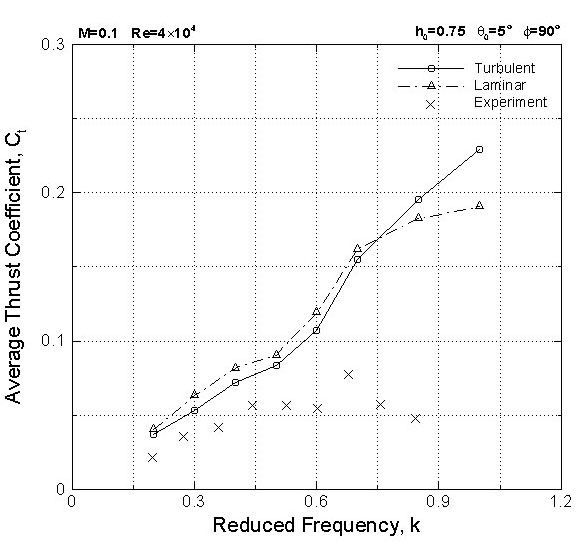
\includegraphics[max height=10cm]{figures/good_plot.jpg}
        % Note that in above figure file name is "good_plot.jpg", and
        % it is located in a directory named "figures".
        \caption{Every figure MUST have a caption. This is an example of \textbf{good} plot.}
                \label{fig:goodplot}
                % The label is used to reference the figure in your text.
                % Things like fig: are optional in the label but it helps
                % to orient yourself when you have multiple figures,
                % equations and tables.
\end{figure}

\begin{figure}[ht] 
        \centering 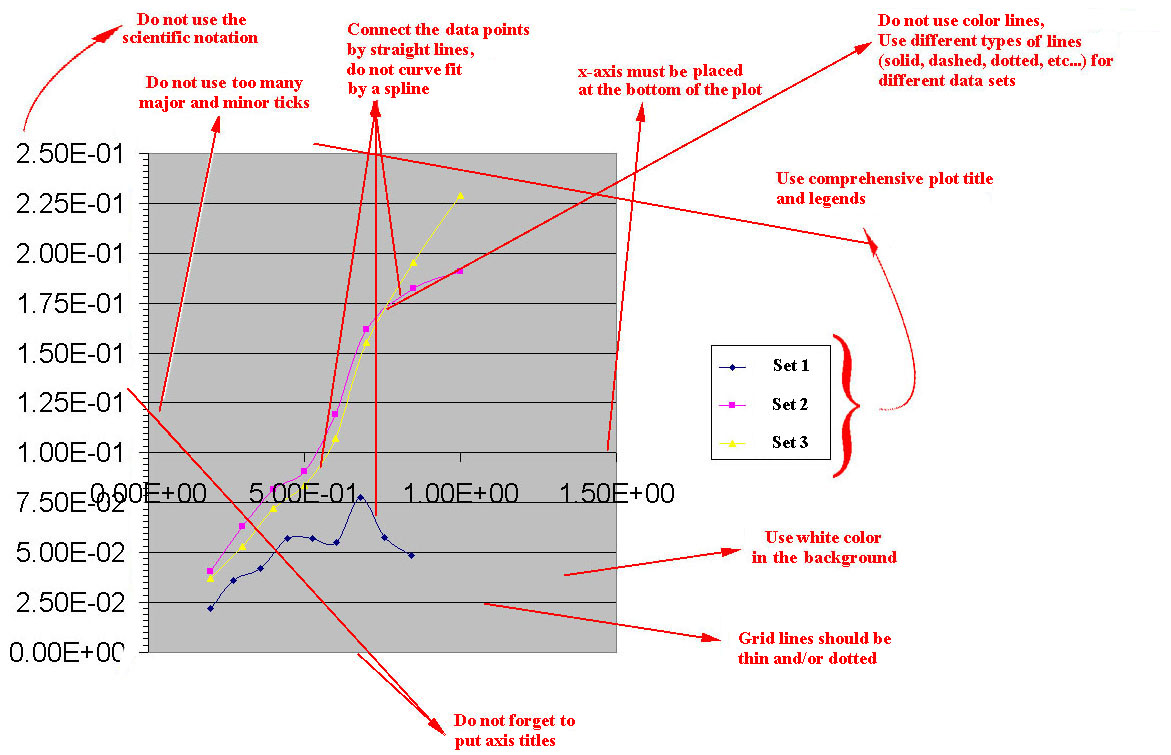
\includegraphics[max height=10cm]{figures/bad_plot.jpg}
        \caption{This is an example of \textbf{bad} plot.}
                \label{fig:badplot}
\end{figure}

Results should be presented in compact graphs with proper, readable legends and captions (see
Figure \ref{fig:goodplot}). Avoid the common mistakes in preparing graphs (see
Figure \ref{fig:badplot}). Again, do not include numerical data tables!

After each finding (e.g. figure), do not forget to explain what you observe
\textit{in that specific result} briefly. Save your general conclusions and comparisons
to the conclusion section.

\subsection{e.g. Write the other method name}

Here is another subsection.

\section{Conclusion}

Finally, conclude your study with comparisons and discussions considering your results.

 \textbf{Conclusion section should be about HALF a page.}

{\vspace{1cm}\Huge DO NOT PUT YOUR CODE IN THE REPORT.} You will submit your code as a separate plain text file on ODTUCLASS.

\end{document}